\documentclass[landscape]{article}
\usepackage[pdftex]{graphicx,color}
\pagestyle{empty}
\oddsidemargin  -0.5 in
\evensidemargin -0.5 in
\headheight     0 in
\topmargin      -1 in
\textheight     7.7 in
\textwidth      10 in
\begin{document}
\Large
\renewcommand{\labelitemi}{-}
\setlength{\parindent}{0 cm}

\begin{center}
  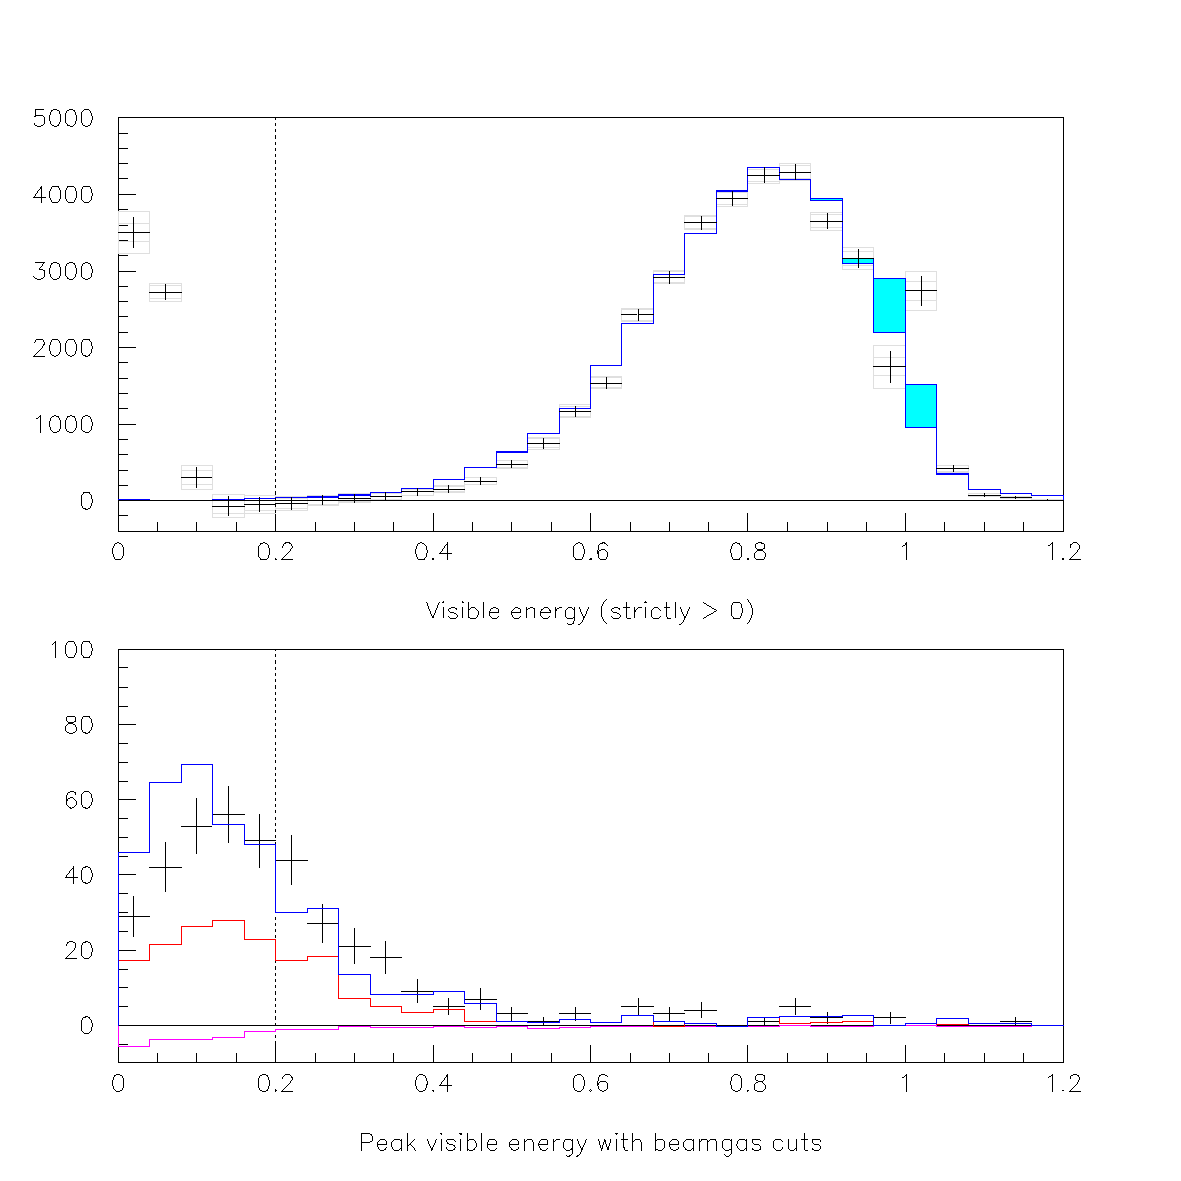
\includegraphics[height=\textheight]{tr2_bgvisen.pdf}
\end{center}

\begin{center}
  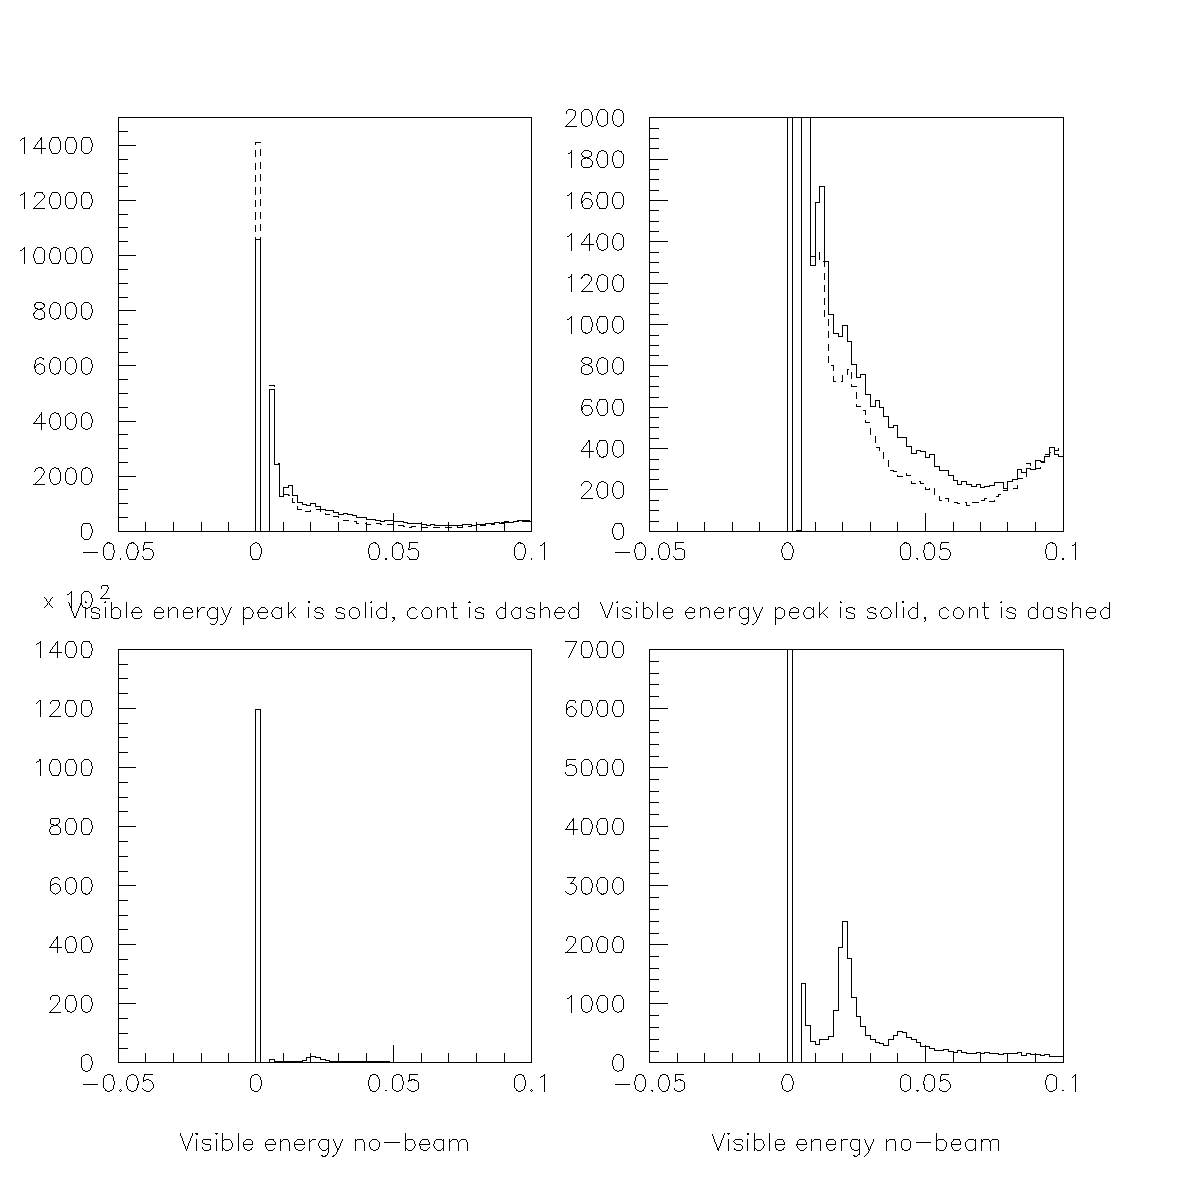
\includegraphics[height=\textheight]{tr2_visen_netherregions.pdf}
\end{center}

\begin{center}
  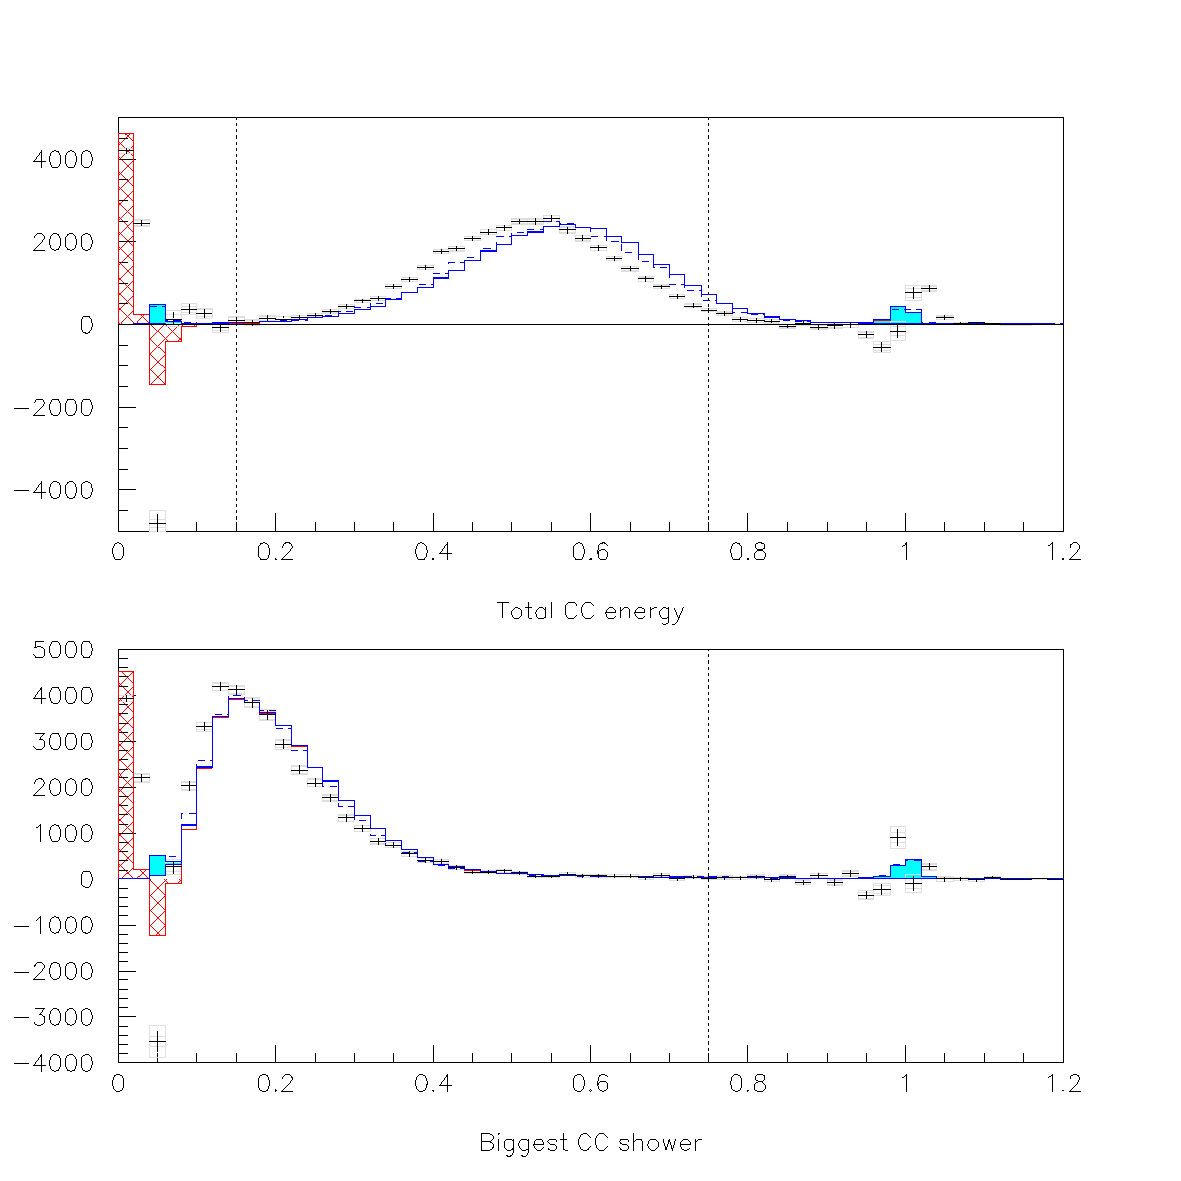
\includegraphics[height=\textheight]{tr2_cc_before_visen.pdf}
\end{center}

\begin{center}
  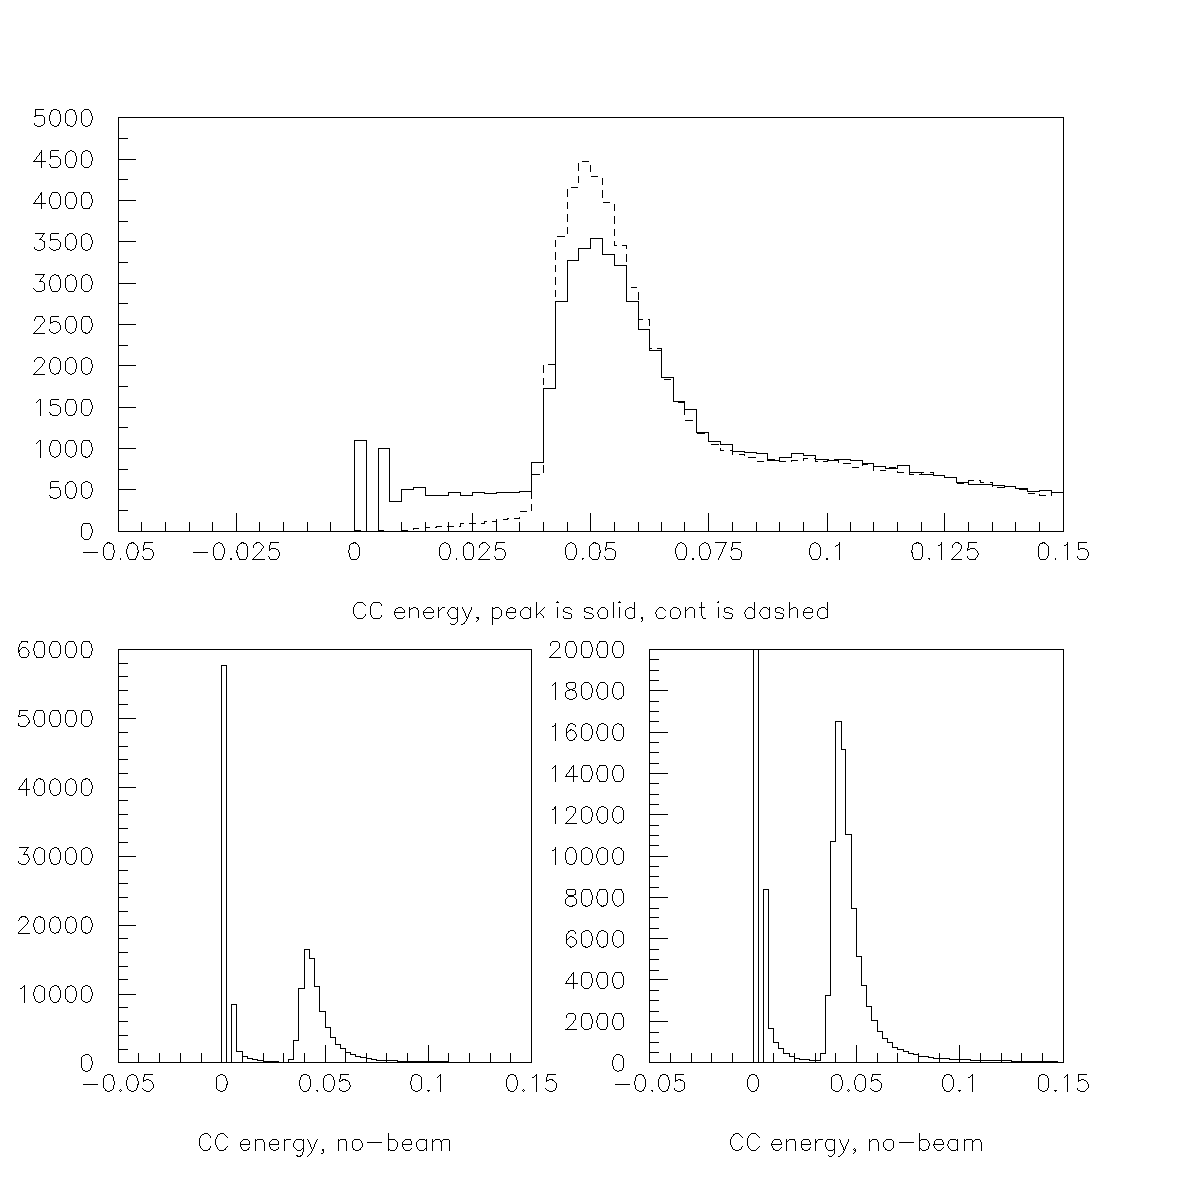
\includegraphics[height=\textheight]{tr2_cc_netherregions.pdf}
\end{center}

\begin{center}
  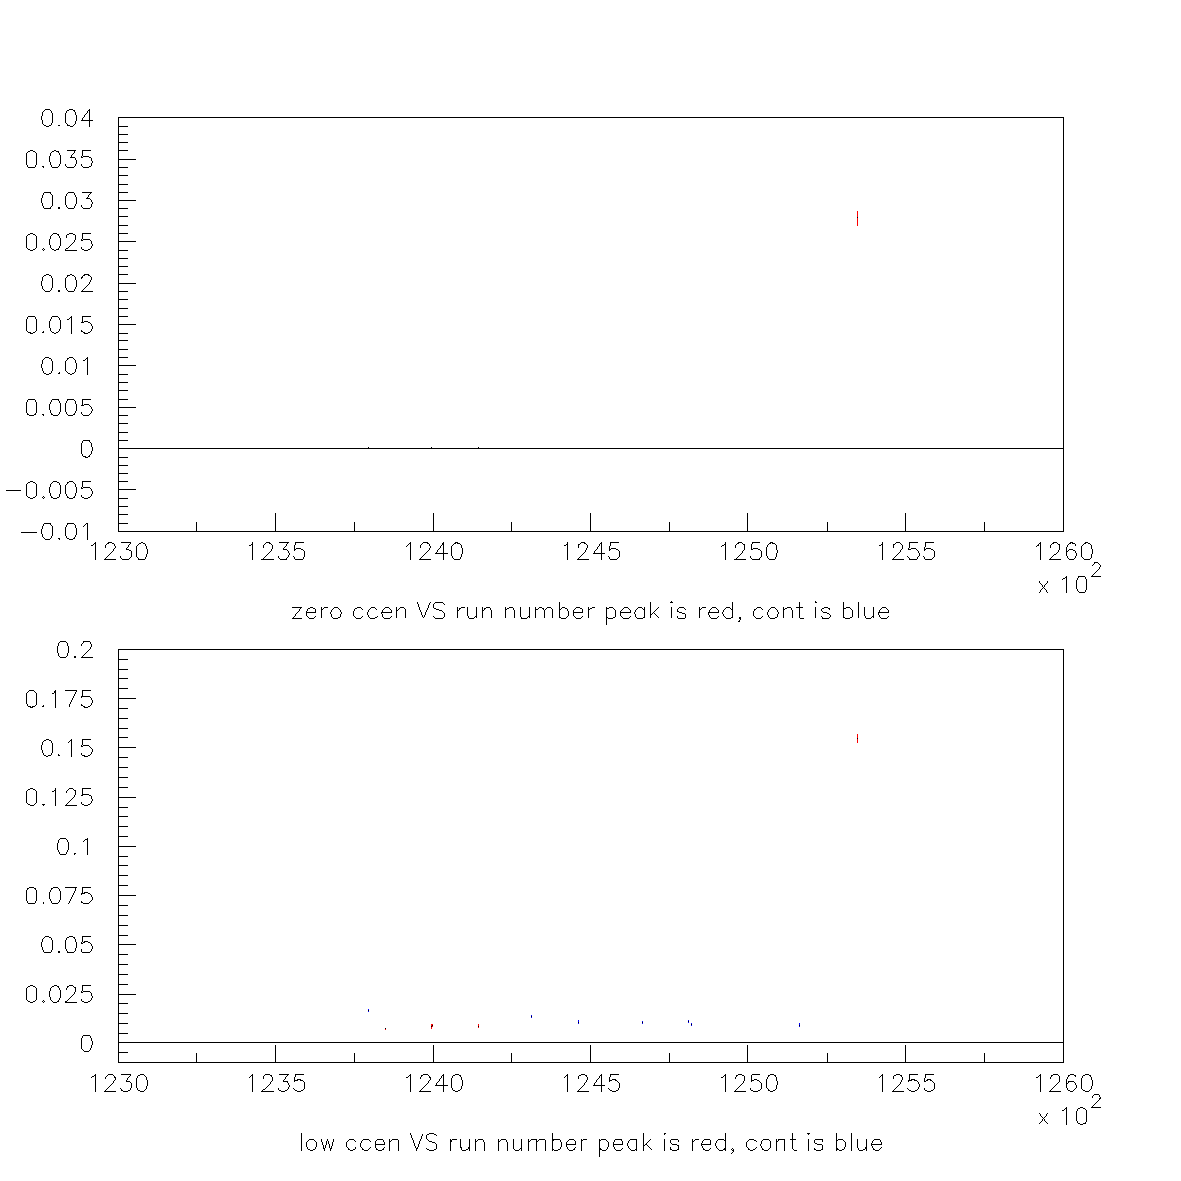
\includegraphics[height=\textheight]{tr2_nether_v_run.pdf}
\end{center}

\begin{center}
  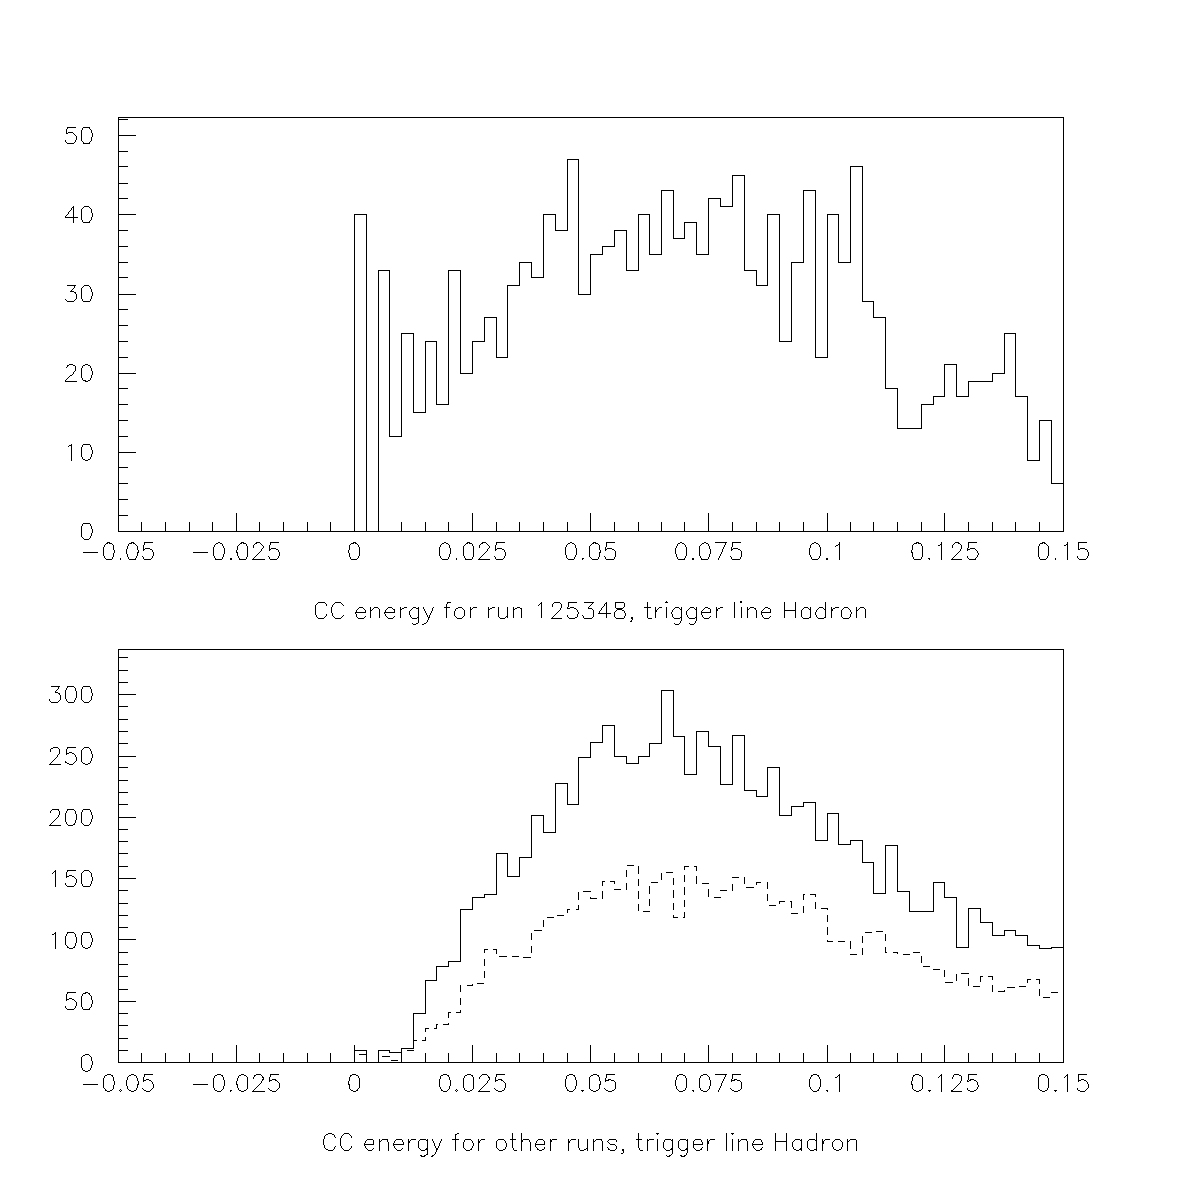
\includegraphics[height=\textheight]{tr2_nether_hadron.pdf}
\end{center}

\begin{center}
  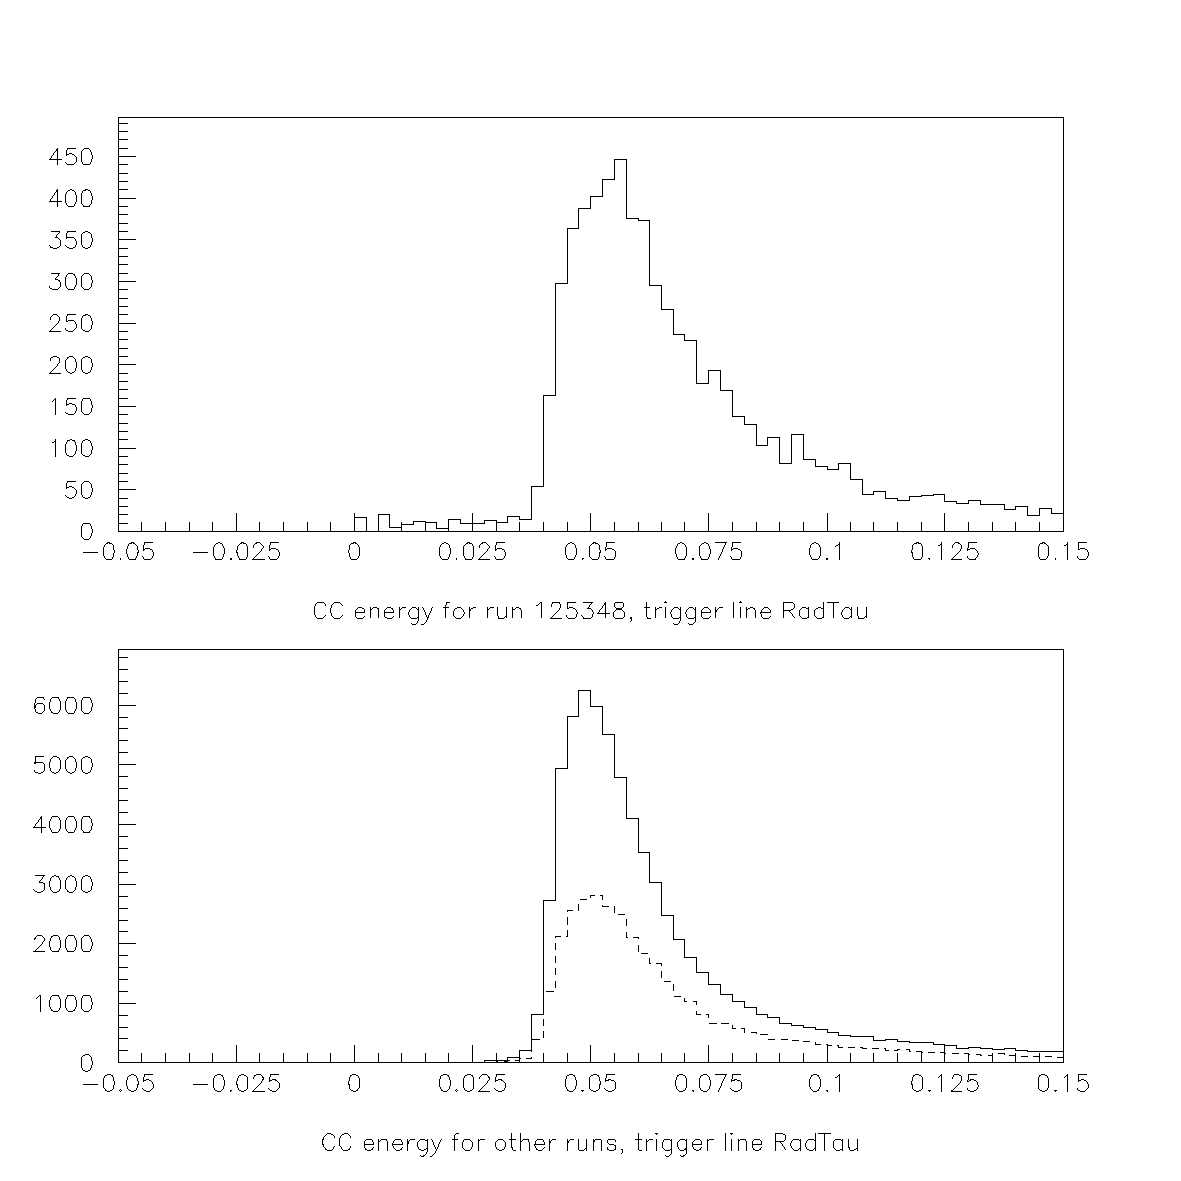
\includegraphics[height=\textheight]{tr2_nether_radtau.pdf}
\end{center}

\begin{center}
  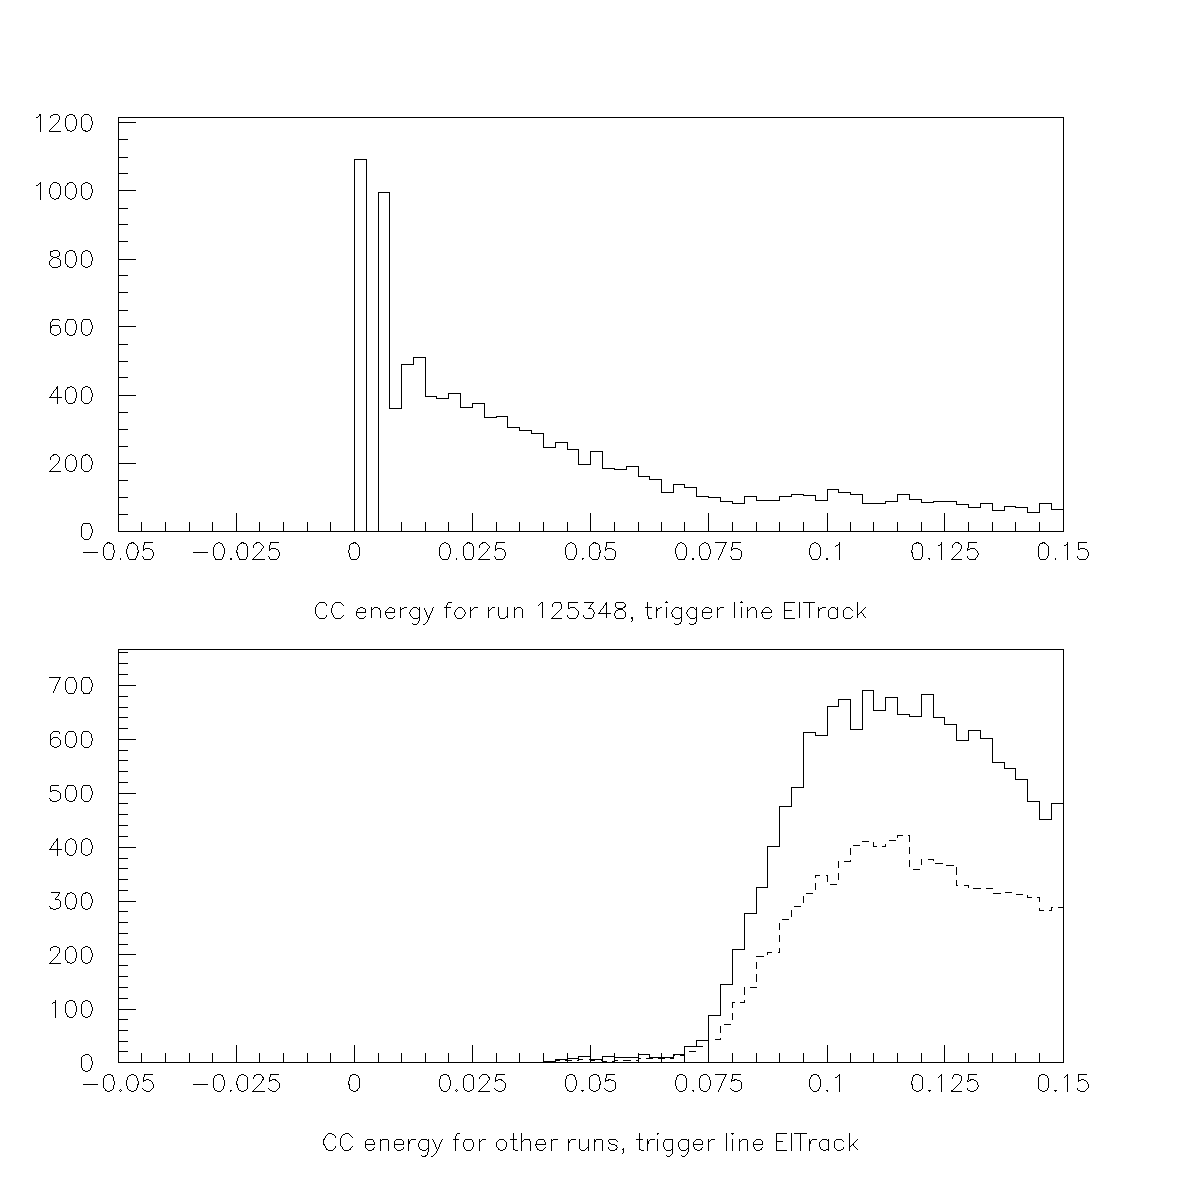
\includegraphics[height=\textheight]{tr2_nether_eltrack.pdf}
\end{center}

\begin{center}
  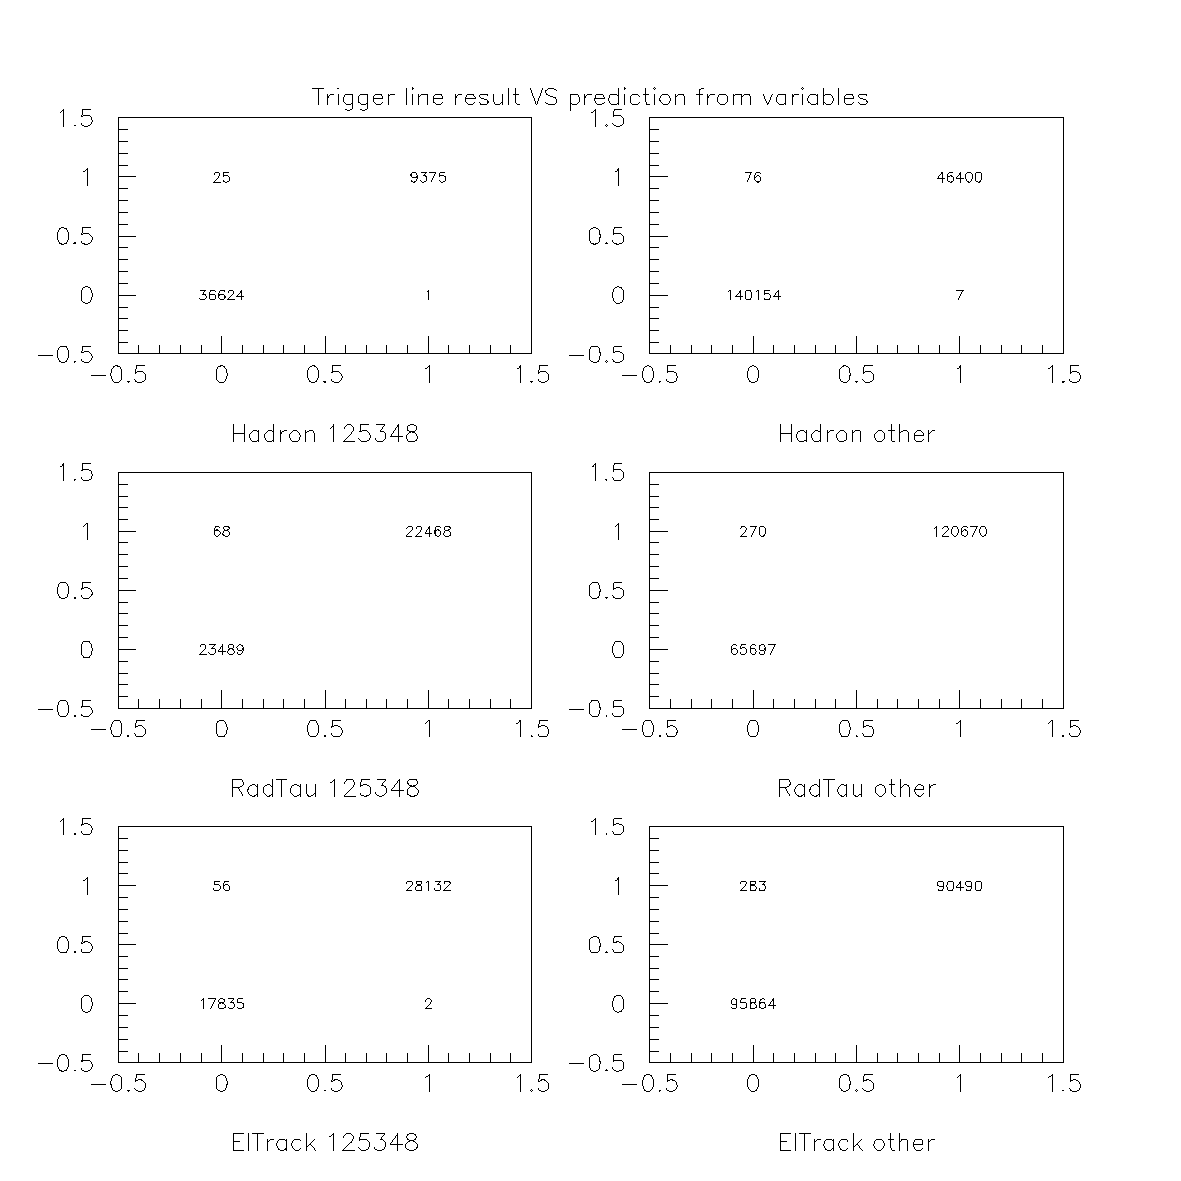
\includegraphics[height=\textheight]{tr2_triggerlines_ok.pdf}
\end{center}

\begin{center}
  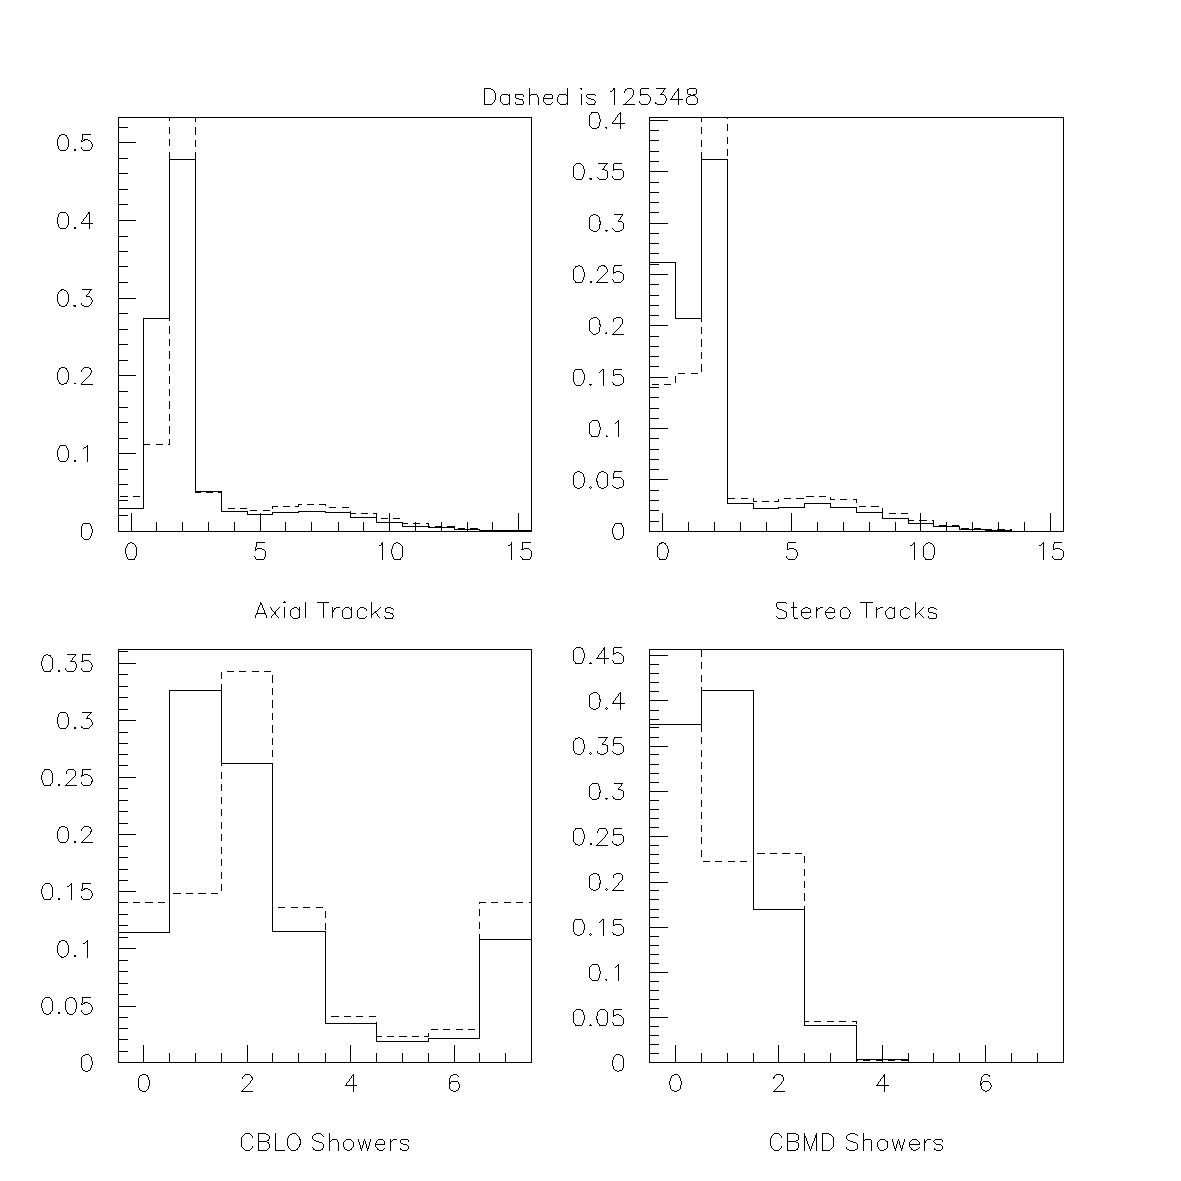
\includegraphics[height=\textheight]{tr2_triggervars.pdf}
\end{center}

\pagebreak

\mbox{ }

\vfill

\begin{center}
\Huge And now back to our regularly-scheduled plots\ldots
\end{center}

\vfill

\pagebreak

\begin{center}
  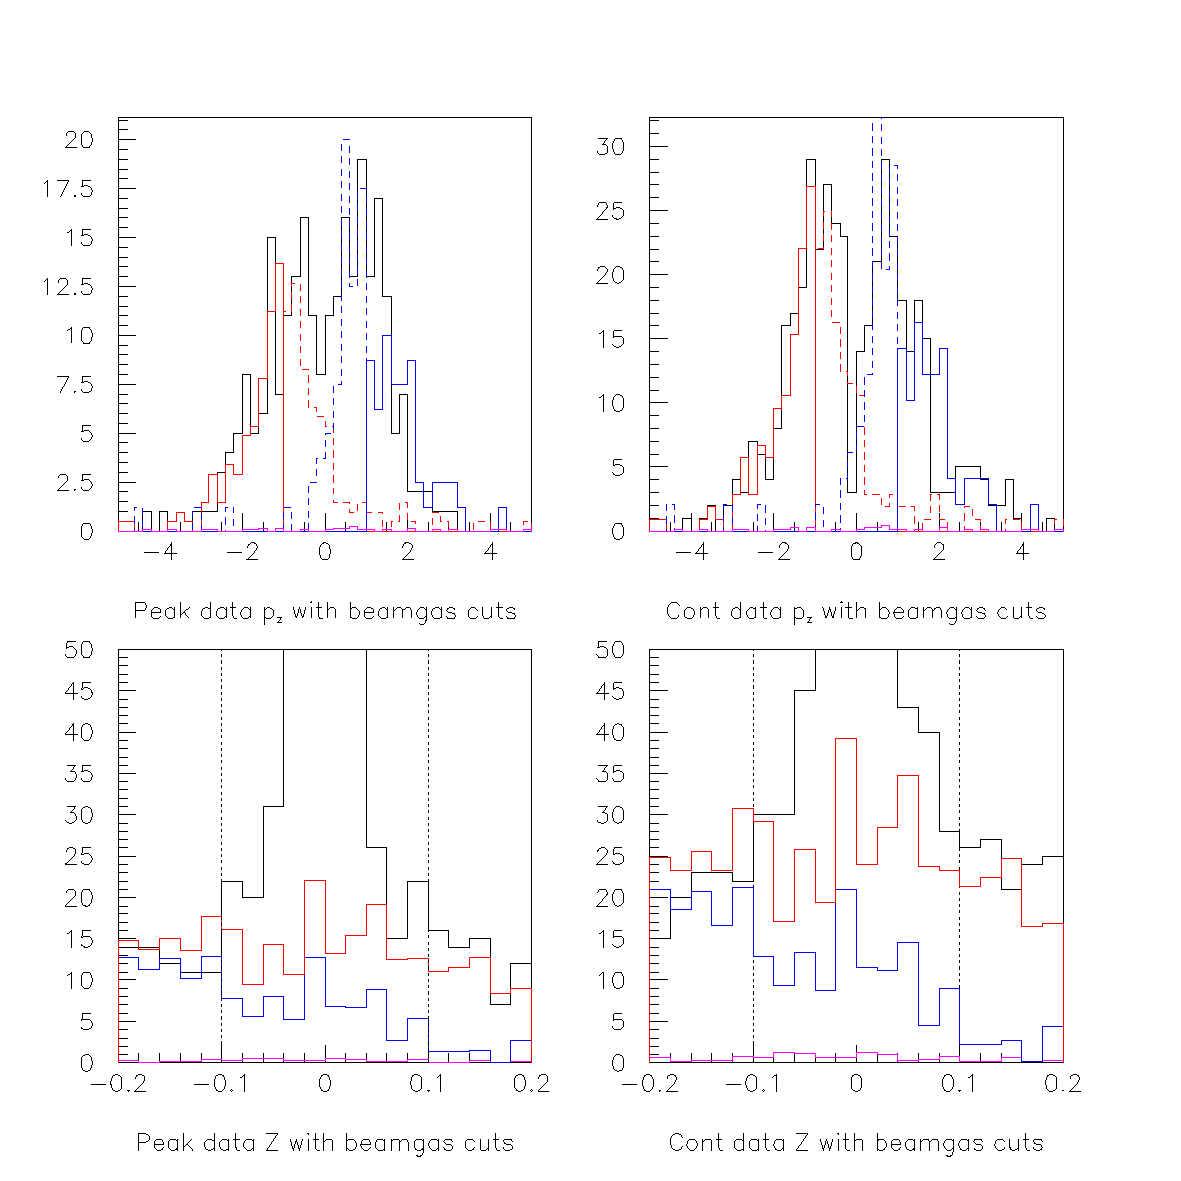
\includegraphics[height=\textheight]{tr2_pctobgep.pdf}
\end{center}

\begin{center}
  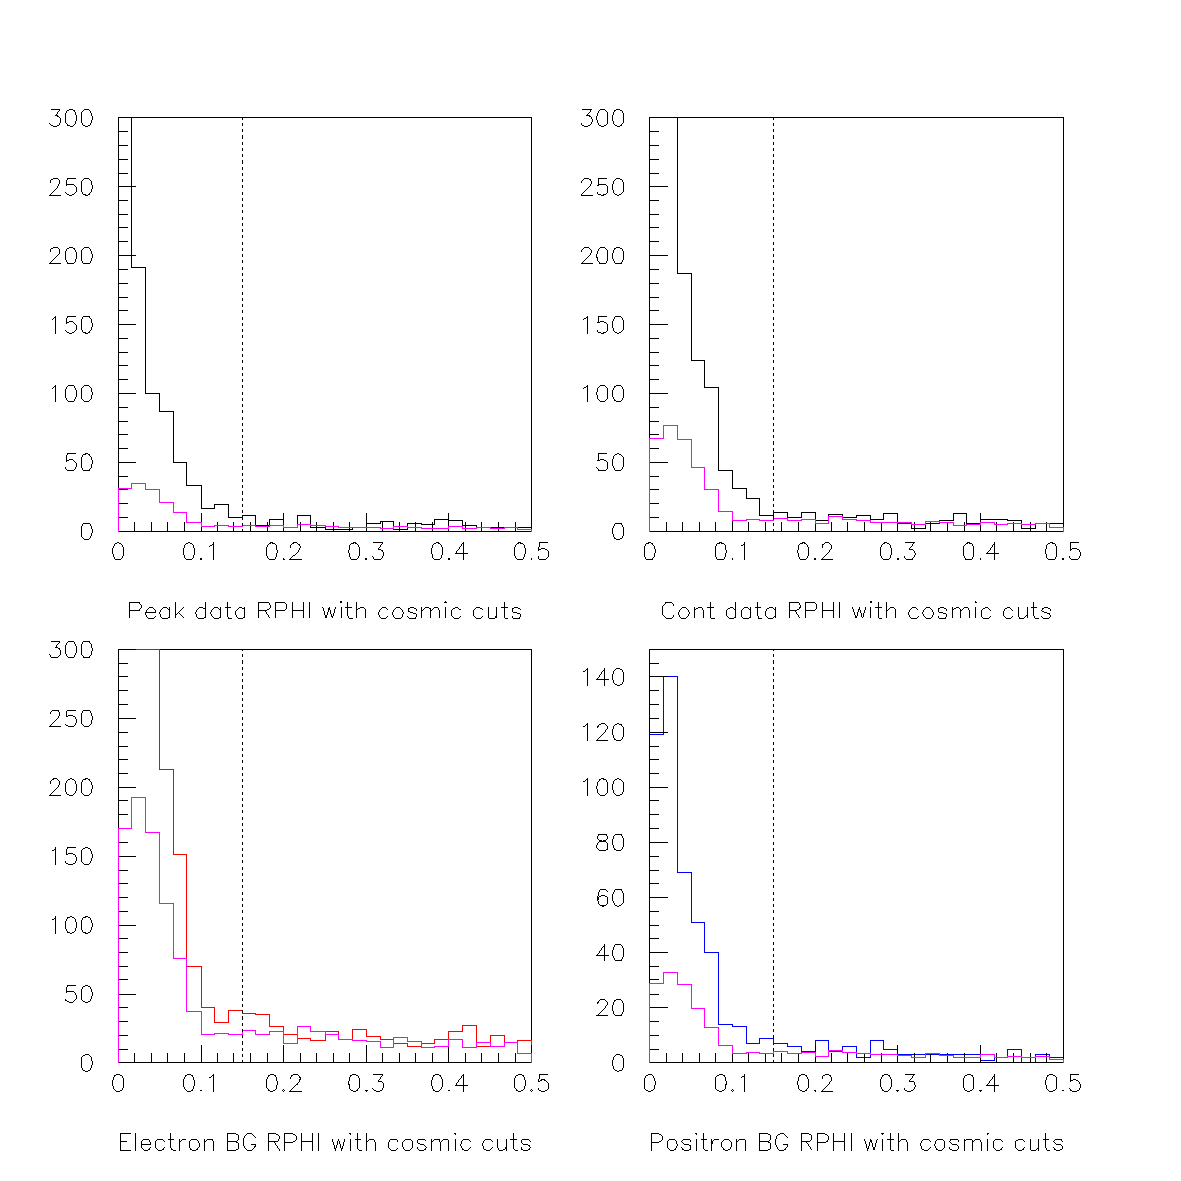
\includegraphics[height=\textheight]{tr2_pcbgepcos.pdf}
\end{center}

\begin{center}
  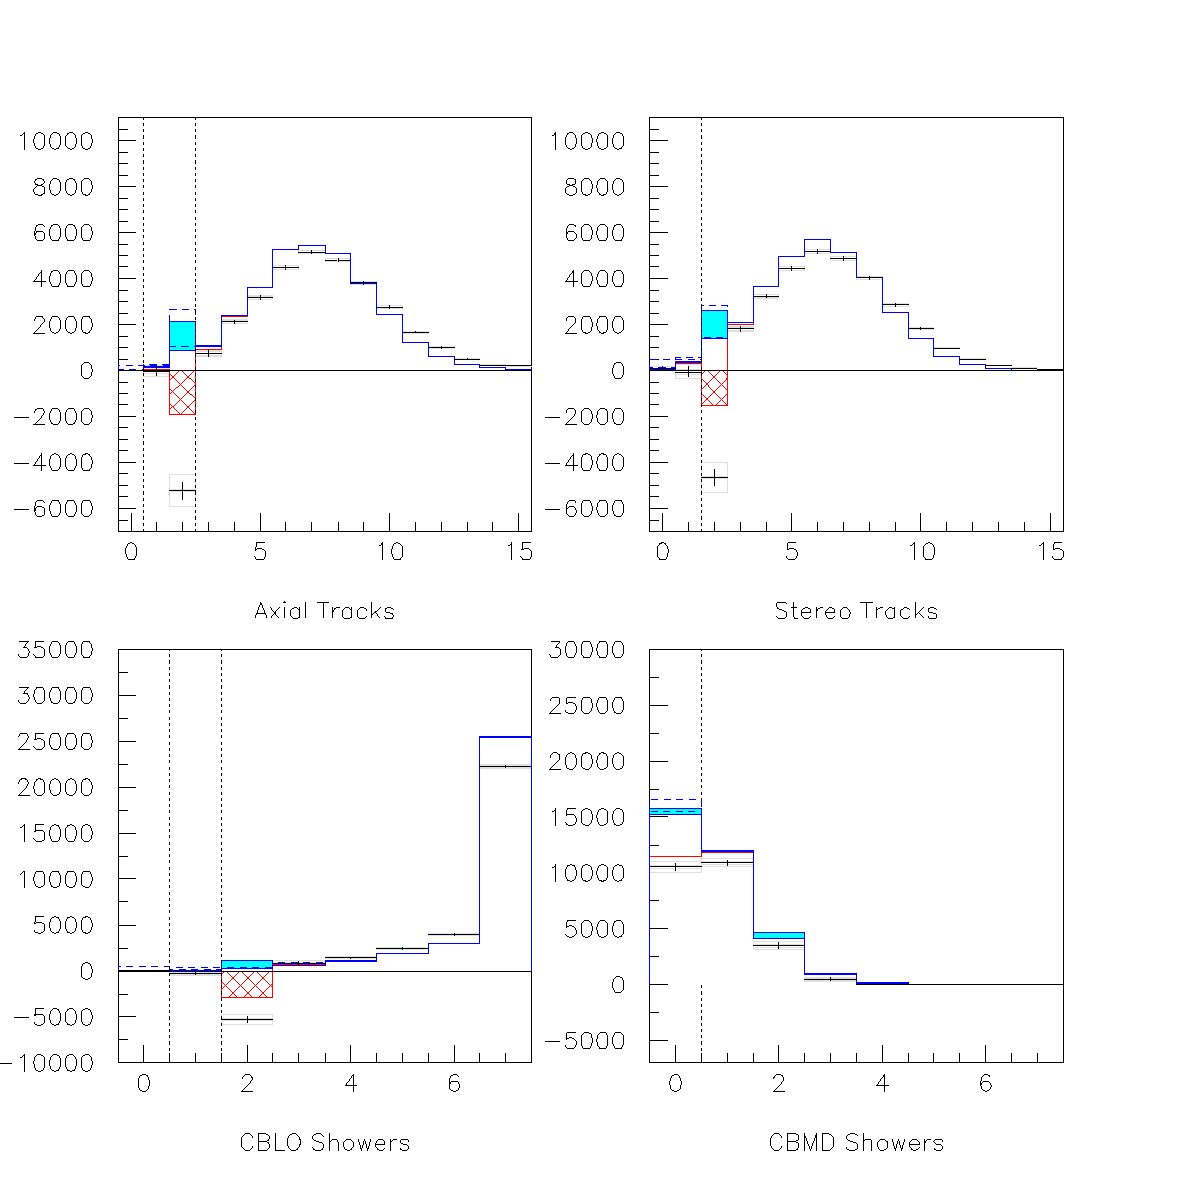
\includegraphics[height=\textheight]{tr2_trigger.pdf}
\end{center}

\begin{center}
  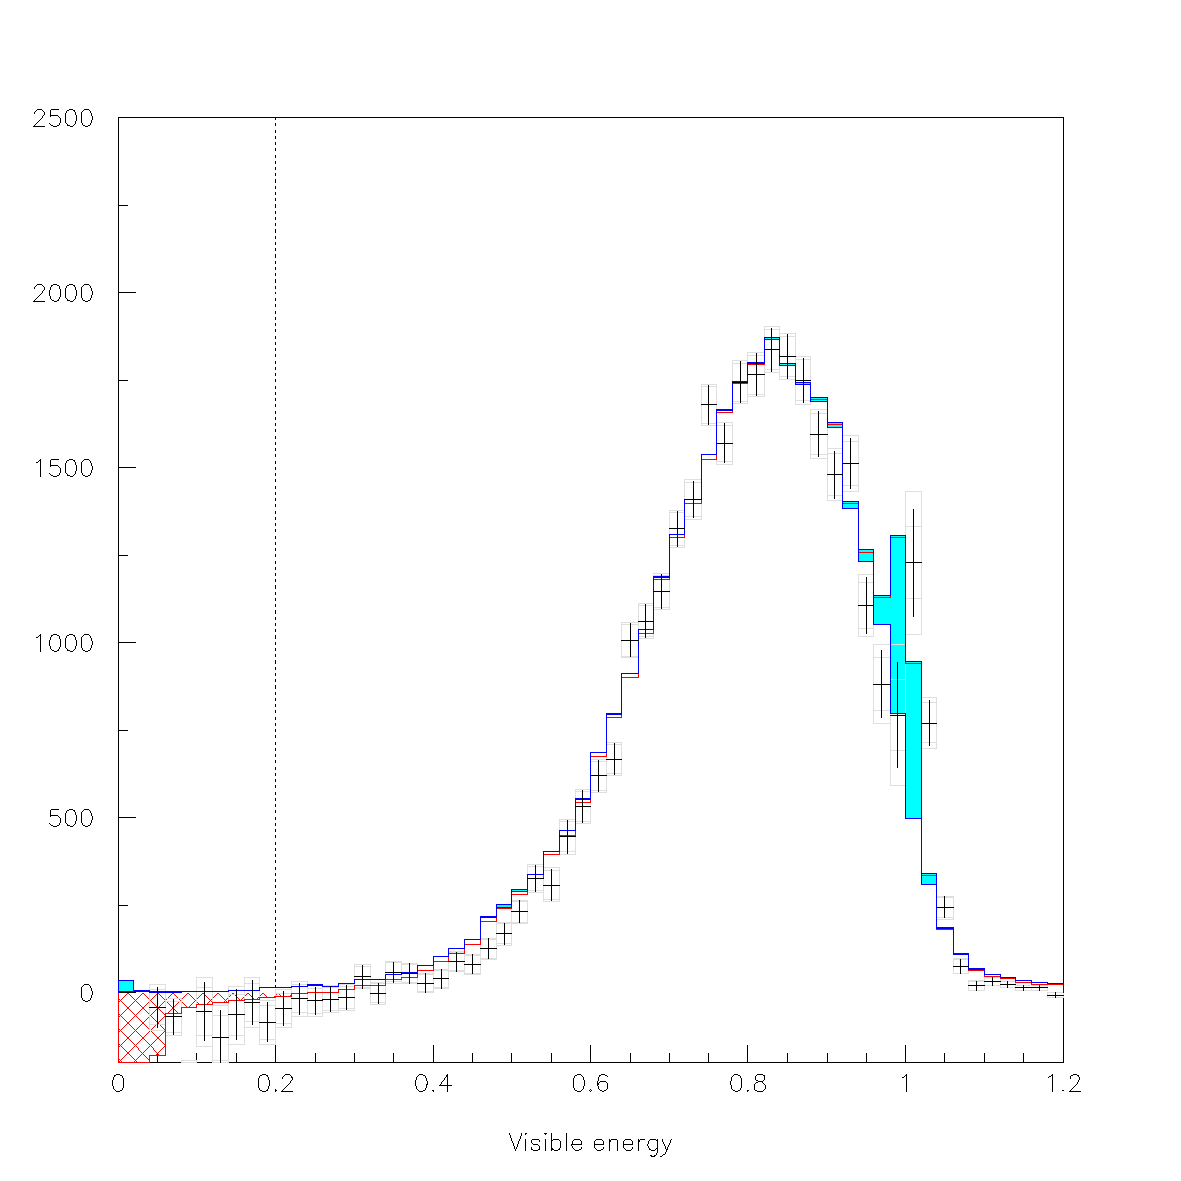
\includegraphics[height=\textheight]{tr2_visen.pdf}
\end{center}

\begin{center}
  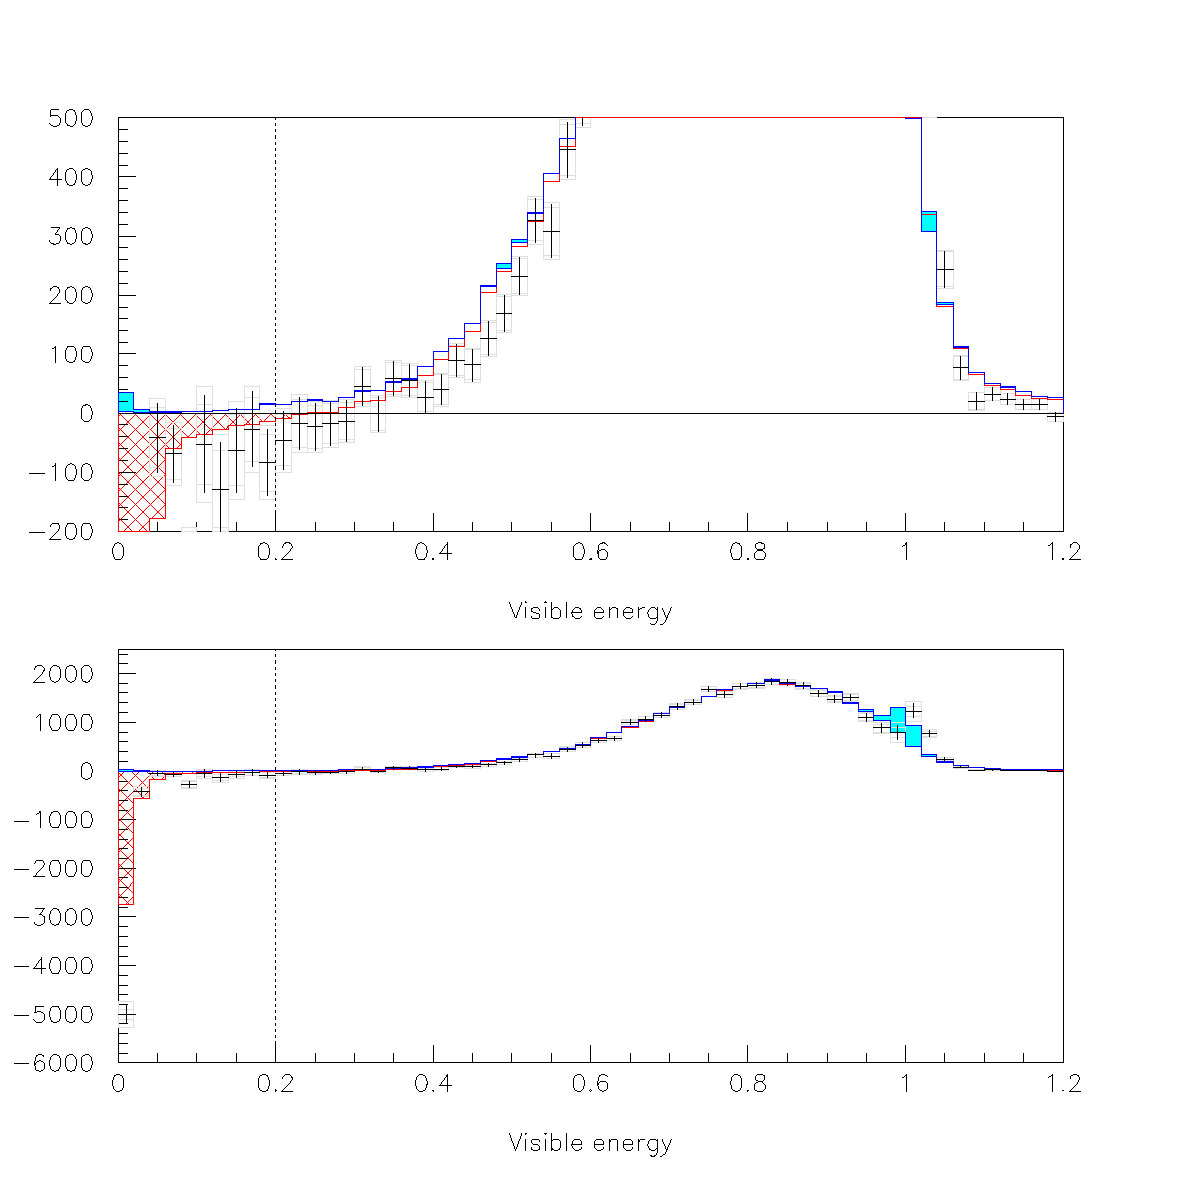
\includegraphics[height=\textheight]{tr2_visen2.pdf}
\end{center}

\begin{center}
  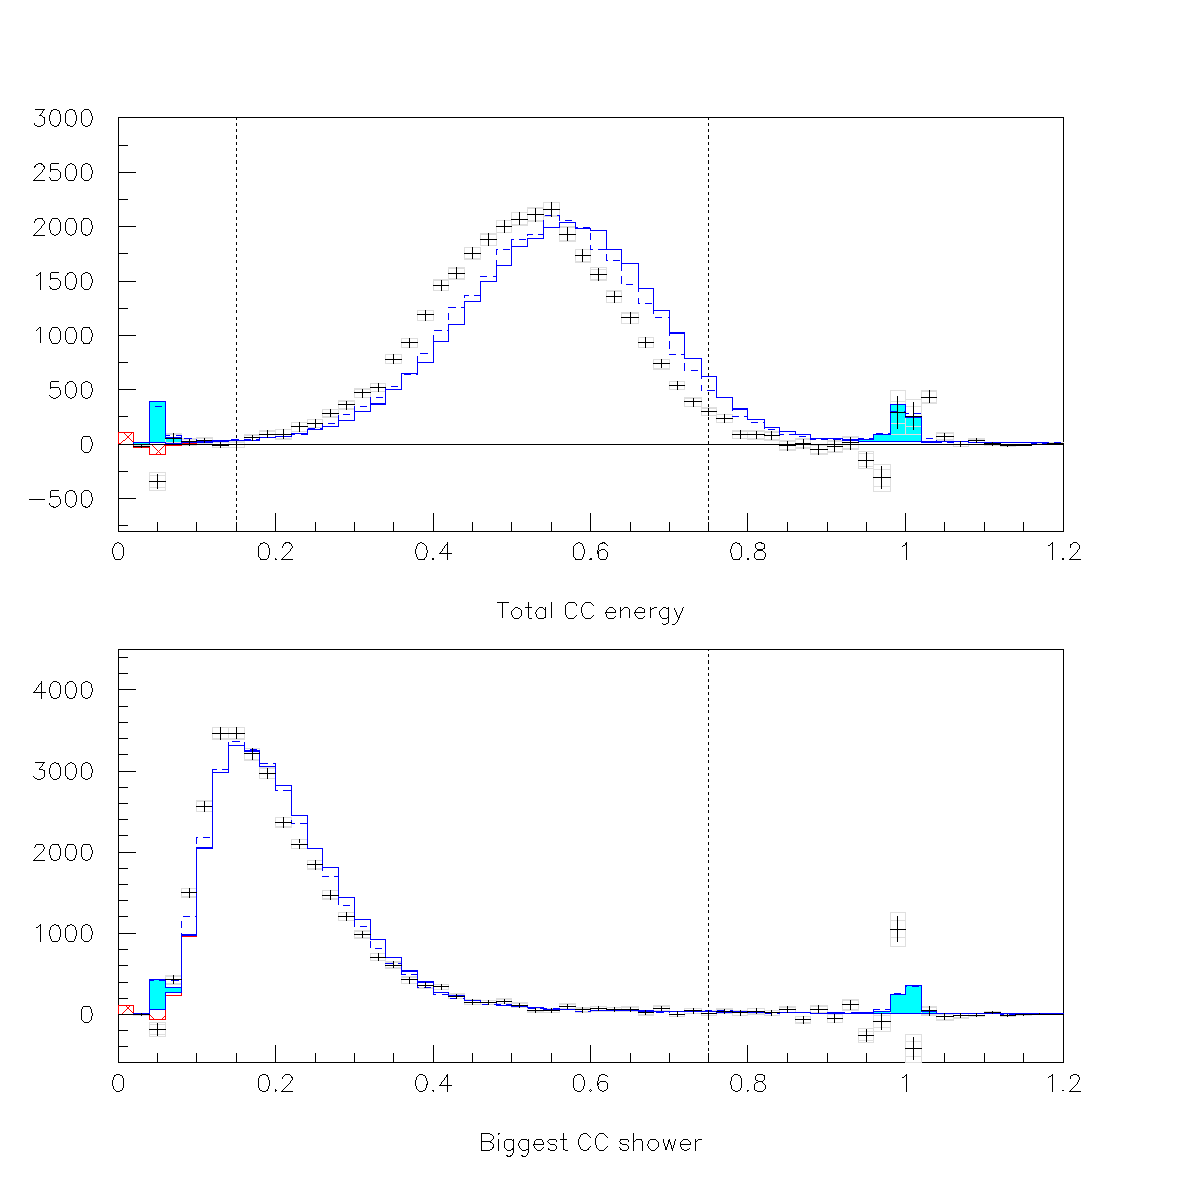
\includegraphics[height=\textheight]{tr2_cc.pdf}
\end{center}

\begin{center}
  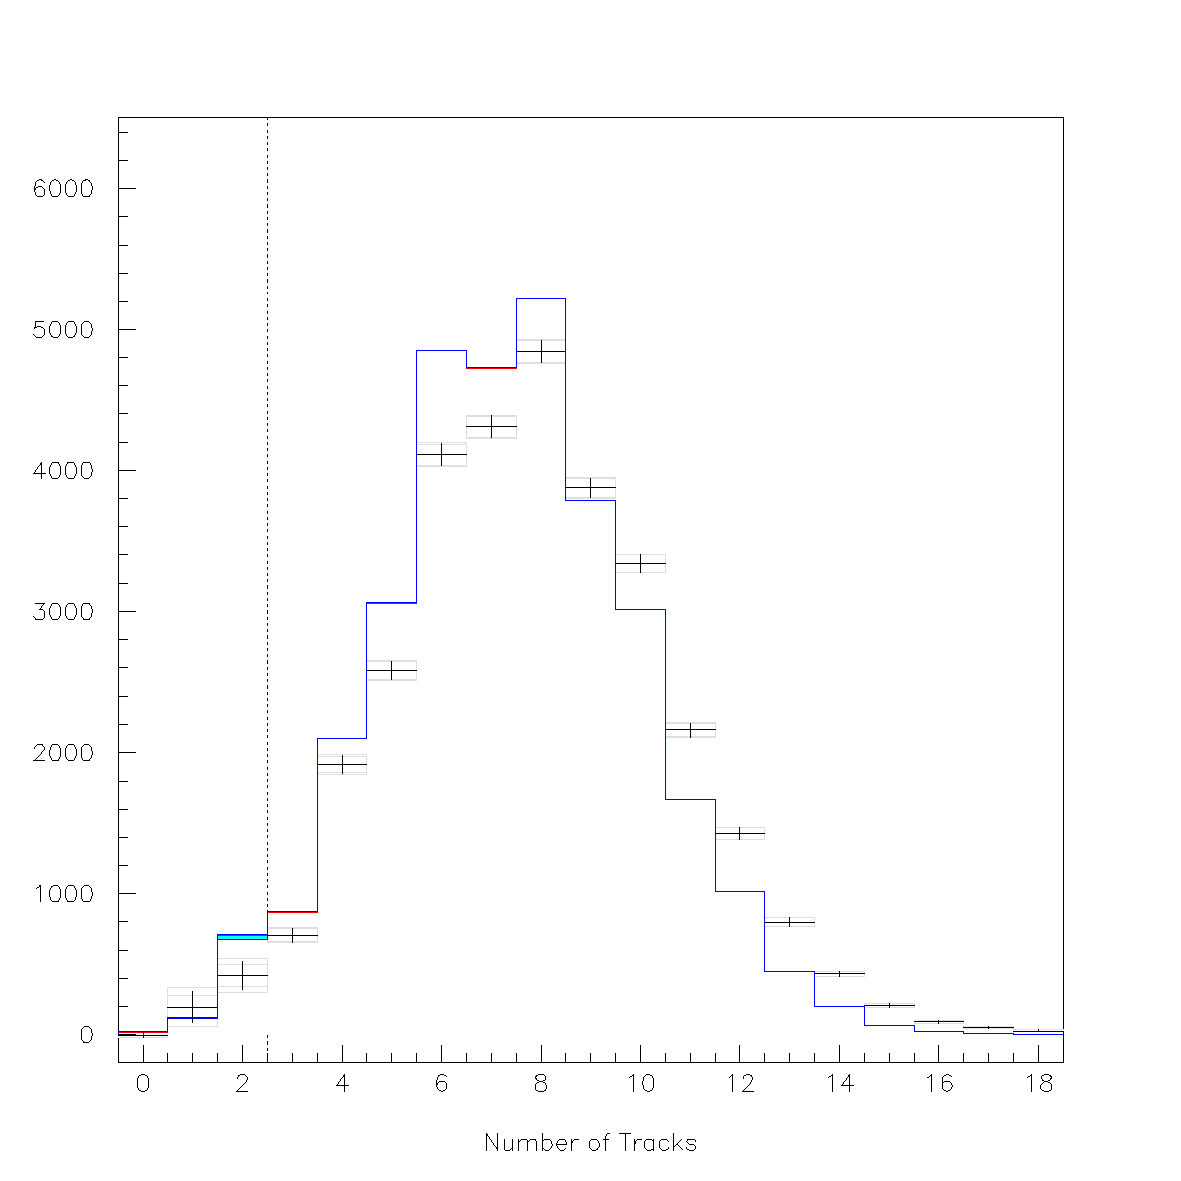
\includegraphics[height=\textheight]{tr2_tracks.pdf}
\end{center}

\begin{center}
  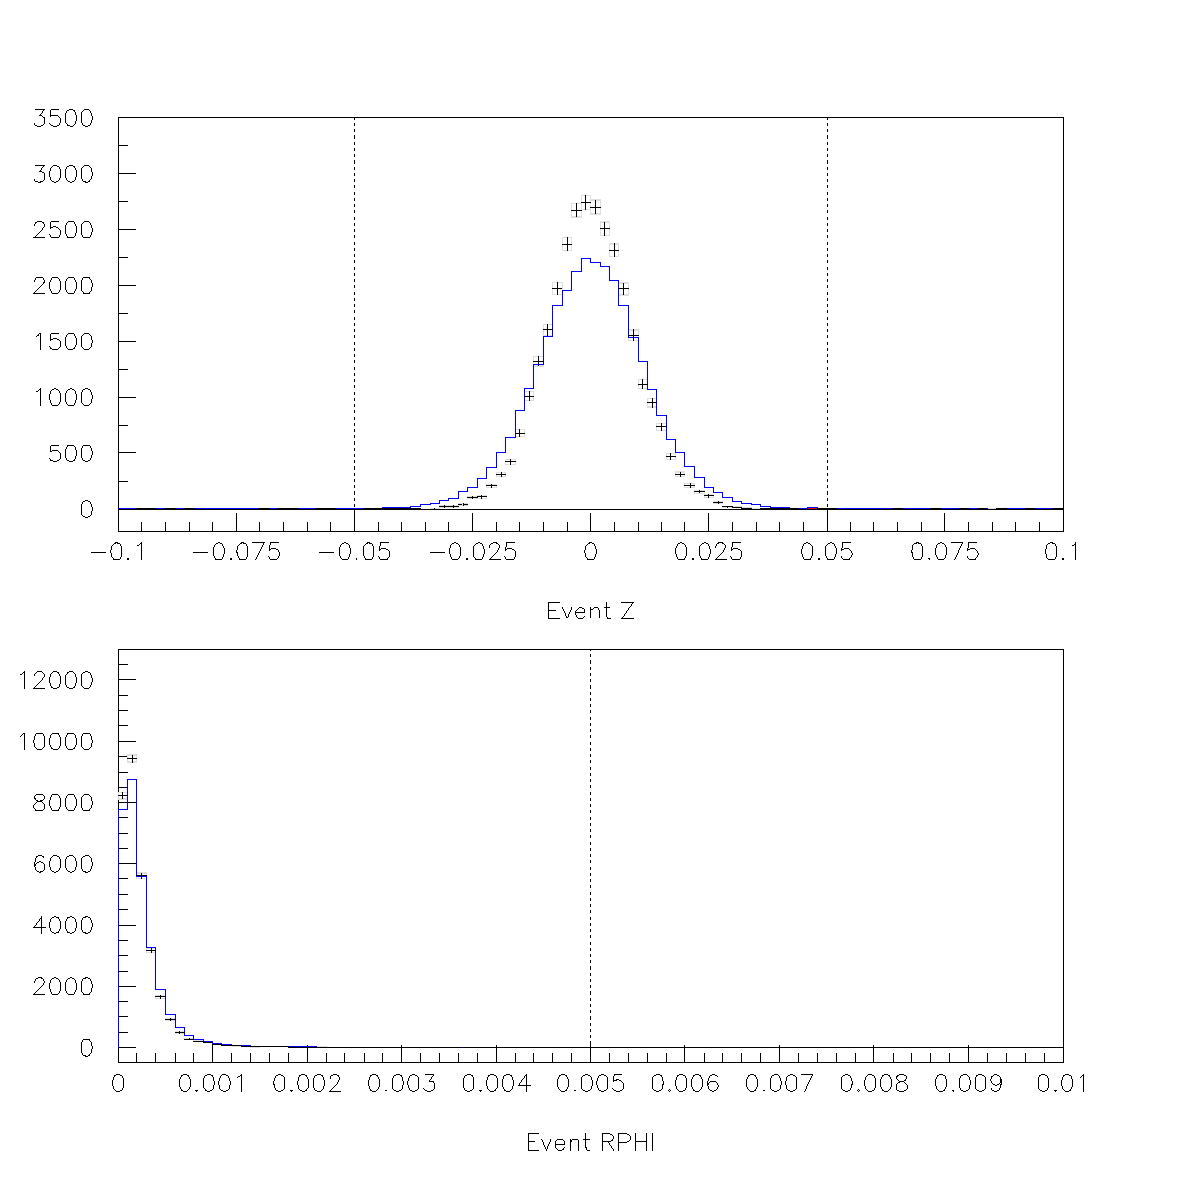
\includegraphics[height=\textheight]{tr2_ciwz.pdf}
\end{center}

\pagebreak

\mbox{ }

\vfill

\section*{Analysis Cuts}

\begin{center}
  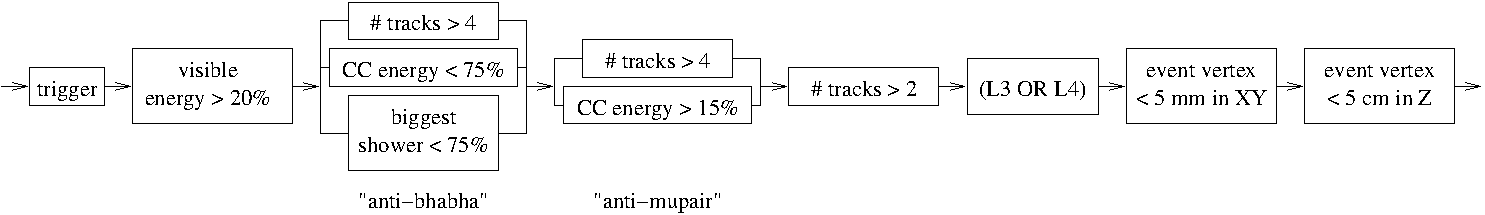
\includegraphics[width=\linewidth]{analysis_cuts.pdf}
\end{center}

\vfill

\section*{Bhabha Cuts}

\begin{center}
  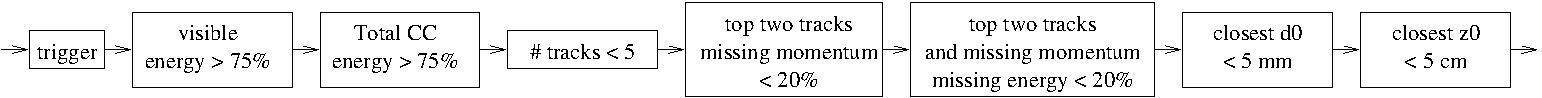
\includegraphics[width=\linewidth]{bhabha_cuts.pdf}
\end{center}

\vfill

\pagebreak

\mbox{ }

\vfill

\begin{center}
{\sc Raw Samples} \\
\vspace{0.2 cm}

\begin{tabular}{l c c c c c c c}
\hline\hline Cuts applied & peak & continuum & $e^-$-beam & $e^-$ BG & $e^+$-beam & $e^+$ BG & Cosmic Rays \\\hline

 trigger & 151819 & 215914 & 150565 & 86354.5 & 31047 & 20102 & 161256 \\
 {\sc and} visible energy $>$ 20\% & 105377 & 126010 & 14879 & 9769.83 & 2415 & 1544.12 & 12831 \\
 {\sc and} anti-bhabha & 58964 & 47371 & 14760 & 9678.7 & 2404 & 1537.87 & 12761 \\
 {\sc and} anti-mupair & 53790 & 38101 & 579 & 495.778 & 159 & 144.814 & 209 \\
 {\sc and} \# tracks $\ge$ 3 & 39438 & 14626 & 176 & 174.805 & 66 & 65.7964 & 3 \\
 {\sc and} level 3, 4 & 39435 & 14619 & 170 & 168.805 & 65 & 64.7964 & 3 \\
 {\sc and} event Z $<$ 5 cm & 39029 & 13972 & 52 & 52 & 19 & 19 & 0 \\
 {\sc and} RPHI $<$ 5 mm (all cuts) & 38823 & 13759 & 24 & 24 & 12 & 12 & 0 \\\hline\hline

\end{tabular}
\end{center}

\vfill

{\small

\begin{center}
\begin{tabular}{c c c}
$\displaystyle \mbox{$\#\Upsilon^a$}_n =
\left(\begin{array}{c}
  \mbox{peak} \\
  \mbox{passing} \\
  \mbox{analysis}
\end{array} \right) -
\left(\begin{array}{c}
  \mbox{cont} \\
  \mbox{passing} \\
  \mbox{analysis}
\end{array} \right)
\begin{array}{c}
  \mbox{ } \\
\underbrace{
\left( \frac{
\left(\begin{array}{c}
  \mbox{peak} \\
  \mbox{passing} \\
  \mbox{bhabha}
\end{array} \right) -
\mbox{$\#\Upsilon^a$}_{n-1}
\displaystyle \left( \frac{\epsilon {\mathcal B}_{\ell\ell}}{\mbox{na\"ive efficiency}} \right)
}{\left(\begin{array}{c}
  \mbox{cont} \\
  \mbox{passing} \\
  \mbox{bhabha}
\end{array} \right)} \right)
} \\
  \mbox{\tt ptoc$_n$} \\
\end{array}
$
&
\begin{minipage}{6 cm}
$\epsilon {\mathcal B}_{\ell\ell}$ = $\displaystyle \frac{\mbox{MC passing bhabha}}{\mbox{MC total}} \mbox{ } \pm \mbox{ 20\%}$ 

\vspace{0.25 cm}
na\"ive efficiency = $\displaystyle \frac{\mbox{MC passing analysis}}{\mbox{MC total}}$
\end{minipage}
&
\begin{minipage}{6 cm}
$a_n = X + Y a_{n-1} \mbox{ and } a_0 = 0$

\vspace{0.25 cm}
$\Rightarrow a_n = \displaystyle \left(\frac{Y^n-1}{Y-1}\right) X$
\end{minipage}

\end{tabular}
\end{center}

}

\vfill

{\large

p = peak, c = continuum, m = Monte Carlo; a = analysis, b = bhabha cuts \\
\{p,c,m\} passing \{a,b\} = data - $e^-$bg scale ($e^-$beam - cosmics) - $e^+$bg scale ($e^+$beam - cosmics) - cosmics scale (no-beam) \\

 ${\tt pa}  = 38823 - 0.488 * ( 24 - 0.39819 * 0 ) - 1.25 * ( 12 - 0.0678733 * 0 ) - 0.0723982 * 0 = 38796.3 $ \\
 ${\tt pb}  = 32958 - 0.488 * ( 0 - 0.39819 * 0 ) - 1.25 * ( 0 - 0.0678733 * 0 ) - 0.0723982 * 0 = 32958 $ \\
 ${\tt ca}  = 13759 - 0.96 * ( 24 - 0.39819 * 0 ) - 2.03846 * ( 12 - 0.0678733 * 0 ) - 0.158371 * 0 = 13711.5 $ \\
 ${\tt cb}  = 55345 - 0.96 * ( 0 - 0.39819 * 0 ) - 2.03846 * ( 0 - 0.0678733 * 0 ) - 0.158371 * 0 = 55345 $ \\
 ${\tt ma}  = 92963 $ \\
 ${\tt mb}  = 1727 $ \\
 ${\tt m2a} = 23792 $ \\
 ${\tt ptoc\mbox{ }\mbox{ }}   = ( 38796.3 * 1.0 * 1727 / 92963 - 32958 ) / ( 13711.5 * 1.0 * 1727 / 92963 - 55345 ) = 0.585172 $ \\
 ${\tt ptocup} = ( 38796.3 * 1.2 * 1727 / 92963 - 32958 ) / ( 13711.5 * 1.2 * 1727 / 92963 - 55345 ) = 0.583094 $ \\
 ${\tt ptocdo} = ( 38796.3 * 0.8 * 1727 / 92963 - 32958 ) / ( 13711.5 * 0.8 * 1727 / 92963 - 55345 ) = 0.587245 $ \\
 ${\tt ptomc}  = ( 38796.3 - 32958 * 13711.5 / 55345 ) / ( 92963 - 1727 * 13711.5 / 55345 ) = 0.331021 $ \\
 ${\tt ptomc2} = ( 38796.3 - 32958 * 13711.5 / 55345 ) / ( 1. - ( 13711.5 / 55345 ) * ( 1727 / 92963 ) ) / 23792 = 1.29341 $ \\


}

\vfill

\pagebreak

\mbox{ }

\vfill

\begin{center}
{\sc Resonance Events Only} \\
\vspace{0.2 cm}

\begin{tabular}{l c c c c c}
\hline\hline Cuts applied & MC$\ell\ell$ & MCother & data & lumi+1$\sigma$ & lumi-1$\sigma$ \\\hline

 none & 5477 & 98493 \\
 trigger & 3784 & 97651 & 25472.1 & 25920.8 & 25024.5 \\
 {\sc and} visible energy $>$ 20\% & 3661 & 97515 & 31639.5 & 31901.4 & 31378.3 \\
 {\sc and} anti-bhabha & 1558 & 96589 & 31243.9 & 31342.2 & 31145.6 \\
 {\sc and} anti-mupair & 124 & 96313 & 31494.3 & 31573.5 & 31415.4 \\
 {\sc and} \# tracks $\ge$ 3 & 3 & 93848 & 30879.3 & 30909.7 & 30848.9 \\
 {\sc and} level 3, 4 & 3 & 93841 & 30880.4 & 30910.8 & 30850.1 \\
 {\sc and} event Z $<$ 5 cm & 3 & 93258 & 30853 & 30882 & 30824 \\
 {\sc and} RPHI $<$ 5 mm (all cuts) & 2 & 92961 & 30771.6 & 30800.2 & 30743.1 \\\hline\hline

\end{tabular}
\end{center}
 
\vfill

\begin{center}
{\sc Samples Scaled To Data} \\
\vspace{0.2 cm}
\begin{tabular}{l c c c c c c}
\hline\hline Cuts applied & MC$\ell\ell$ & MCother & data & $e^-$ BG & $e^+$ BG & Cosmic Rays \\\hline

 none & 1812.97 & 32603.3 \\
 trigger & 1252.6 & 32324.5 & 25472.1 & -6369.92 & 1148.83 & 841.332 \\
 {\sc and} visible energy $>$ 20\% & 1211.83 & 32279.5 & 31639.5 & -720.669 & 88.2464 & 66.9441 \\
 {\sc and} anti-bhabha & 515.801 & 31973 & 31243.9 & -713.947 & 87.8894 & 66.5789 \\
 {\sc and} anti-mupair & 41 & 31881.6 & 31494.3 & -36.571 & 8.27616 & 1.09043 \\
 {\sc and} \# tracks $\ge$ 3 & 1 & 31065.6 & 30879.3 & -12.8945 & 3.76027 & 0.0156521 \\
 {\sc and} level 3, 4 & 1 & 31063.3 & 30880.4 & -12.4519 & 3.70311 & 0.0156521 \\
 {\sc and} event Z $<$ 5 cm & 0.929687 & 30870.4 & 30853 & -3.83577 & 1.08585 & 0 \\
 {\sc and} RPHI $<$ 5 mm (all cuts) & 0.699219 & 30772 & 30771.6 & -1.77036 & 0.685801 & 0 \\\hline\hline

(last line constraint) & A & + B & = C & $-$ D & $-$ E & $-$ F \\

\end{tabular}
\end{center}

\vfill

\end{document}
